%\section{Power Model Dependency on App Usage - A TPMD Study}
%\section{At What Granularity of App Run Should We Apply SPMD?}
\section{Drawbacks of TPMD}
\label{sec:primer}

% Since SPMD is meant to capture the power model's dependence on app usage, it should be applied to 
% each app run interval that exhibits the {\em same} component usage.
% To gain insight into the extent of such "same" component usage intervals of apps,
% we start with a study to find out  how much the GPU power models derived using TPMD vary with
% apps and app scenarios. 

% show the component power draw dependency on app usage 
% using a representative modern phone, Moto Z3,
% by performing TPMD to generate the CPU and GPU power models
% on a representative modern phone, Moto Z3.
% In particular, we discuss the four-step process of TPMD discussed in \S\ref{sec:back} for the CPU and the GPU.
For the experiments in this section,
we use the external Monsoon power monitor ~\cite{monsoonpowermonitor} to measure the phone power draw.
We keep the screen brightness level at 0 which consumes
43.21 mA, 57.58 mA, and 78.82 mA respectively for the 3 phones; and this is subtracted
from the total phone power draw measurement.

\begin{table}[t]
{\footnotesize
    \centering
    \caption{CPU and GPU power model parameters on the 3 phone. (PF: per frequency.)}
    \vspace{-0.1in}
    \begin{tabular}{|p{2.25cm}|c|c|c|c|}
        \hline
        Model Parameters & Parameter  & \multicolumn{3}{c|}{Number of Parameters}\\
         \cline{3-5}
          & Symbol & Pixel 2 & Moto Z3 & Pixel 4\\
        \hline
        CPU base power                          & $p^c_{\text{base}}$          &  1      &   1       & 1\\
        CPU core $i$ power at freq. $f_k$       & $p^c_i(f_k)$          & 31, PF  &  31, PF   & 17, PF\\
        % TODO: add per frequency per core in the description\\
        GPU busy power at freq. $g_k$           & $p^g_{\text{busy}}(g_k)$     &  7, PF  &   7, PF   & 5, PF\\
        GPU idle power at freq. $g_k$           & $p^g_{\text{idle}}(g_k)$     &  7, PF  &   7, PF   & 5, PF\\
        \hline
    \end{tabular}
    \label{tab:parameters}
    \vspace{-0.2in}
}
\end{table}

% \questionaj{We need a paragraph here (perhaps reference table 3?) detailing which 
% trigger are we logging, where are we logging them from, and is experiment done 
% using power monitor or power sensor


%\if 0
\subsection{Power Model for Modern Smartphones}

The modern smartphones have came a long way, with different components which are capable of running in various power states.
This calls for a complex power model, in comparison to the pure utilization model.
We focus our attention in exploring per-component self-modeling of smartphone using CPU and GPU.
The decision of modeling only CPU and GPU was taken due to the fact that these are major energy consuming components in a modern day smartphones.

\fi
%%% Need to justify with a profiled data

% However earlier paper ~\cite{Zhang2015self} 
% observe  that this
% assumption does not hold good for multicore CPUs in modern smartphones. Even under the same frequency and
% CPU utilization, two workloads with different CPU usage patterns could
% consume significantly different amounts of energy
% The root
% cause of the estimation inaccuracy and instability come
% from multiple newly introduced CPU idle power states,
% which consume markedly different amounts of power in
% multicore CPUs. Workloads with different CPU usage
% patterns cause CPU to enter different idle power states
% during the computation, which in turn leads to different amount of CPU power consumption.

%\subsection{CPU Power Model is App Dependent}
\label{sec:primer_cpu}

%%% Things discussed in this section
%% 1. Explain the CPU architecture
%% 2. Explain how memory operation effects CPU model
%%   2a. Description of benchmark
%%   2b. What we did
%%   2c. Explanation of results
%% 3. Explain how CPU model is derived and generated
%%   3a. What did we do
%%   3b. How model is derived
%%   3c. Explain Base Current and Non-Base Current
%% 4. Explain the complete model

\paragraph{Parameters of a multicore CPU power model}
% 1. Explain the CPU architecture
Moto Z3~\cite{motoz3} is a representative modern smartphone
that uses the big.LITTLE CPU architecture~\cite{biglittlearch} to
provide energy efficiency in supporting diverse workloads.
% In this architecture, the CPU has two core clusters,
% the LITTLE cores with low compute performance and high power efficiency and
% big cores with high performance for processing compute-intensive tasks.
%The use of big.LITTLE cores depends on the dynamic usage pattern of smartphones i.e. when the phone is not working on doing any computationally intensive tasks it switches to LITTLE cores, dramatically extending the battery life.
% The cores in each cluster can run at various frequencies which correspond to 
% different core power states draining different amount of power.
In particular, in Moto Z3, the LITTLE cores can operate in 22 frequencies 
and big cores can operate in 31 frequencies.
%  The cores are switched to higher frequencies when higher performance is required.
At runtime, the OS scheduler along with the CPU governor performs power state transition and core frequency scaling to optimize the CPU energy drain as the workload varies.

Thus the parameters of the CPU power model include
the base power consumed $p_{base}$ when the cores are idle and
the non-base core $i$ power running at frequency $f_k$, $p^c_i(f_k)$, as listed in Table~\ref{tab:parameters}.
The total CPU power can be modeled~\cite{multicoremodel:2015} as follows:
\if 0
Accordingly, we model the CPU power draw as follows:
\begin{equation}
    P_{CPU} = p^c_{base} + \sum_i p^c_i{f(i)}
\end{equation}
where $p_{base}$ denotes the base power consumed when the cores are active and
$p_i{f_k}$ is the non-base power of core $i$ at frequency $f_k$.
\fi
{
\begin{equation}
    P_{CPU} = p^c_{base} + \sum_{i} p^c_i(f_k)
\end{equation}

}

\paragraph{TPMD methodology}
%% Flow of section
% 3. Explain how CPU model is derived and generated
%% 3a. What did we do
To derive the above CPU power model for Moto Z3,
we wrote a microbenchmark program that performs arithmetic-operations for 7 seconds at 100\% utilization followed by memory operations for 7 seconds at 100\% utilization. 
We ran the microbenchmark 10 times while fixing the big core cluster at each of the 31 frequencies, 
on 1 core, 2 cores and 4 cores.
When using 1 core, 2 cores and 4 cores, the remaining cores are offline.
We measure the base CPU power as the phone power draw when all cores are idle.
\footnote{We noticed even when the phone is idle, there are many system processes running in the background.
% 
So we obtained the accurate
base power from extrapolating the measured current vs. utilization curve for each frequency.}
We manually align the power monitor readings with each 7-second interval, 
and derive the non-base per-core power for each frequency by 
subtracting the base power from the measured total phone power.
{On Moto Z3, the per-core power $p_i(f_k)$ remains the same for different cores.}



% panab, check this ---
% The base CPU power is the current at utilization 0 and obtained from extrapolating the measured current vs utilization curve for each frequency.
% The non-base per-core CPU power for each frequency is the slope of the curve as shown in figure~\ref{fig:cpu_model_derivation}.

% at each big frequency.
% Little cores are offline
% Explain observations of microbenchmark

\if 0
\begin{figure}[tp]
    \centering
    \vspace{-0.1in}
         \begin{subfigure}[b]{0.49\columnwidth}
         \centering
         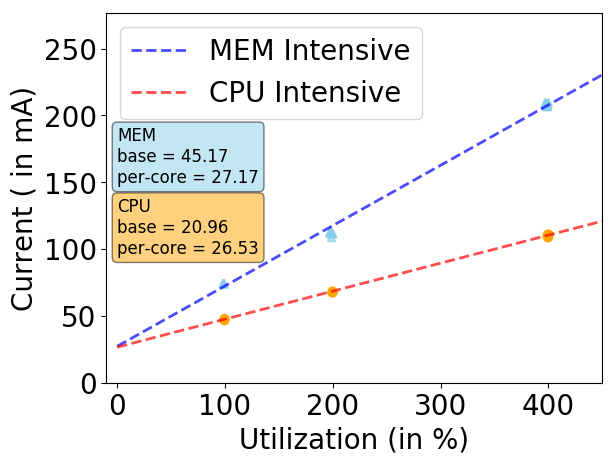
\includegraphics[width=\textwidth]{figures/576000.png}
         \caption{576 MHz}
         \label{fig:cpu_576000}
    \end{subfigure}
    \hfill
    \begin{subfigure}[b]{0.49\columnwidth}
         \centering
         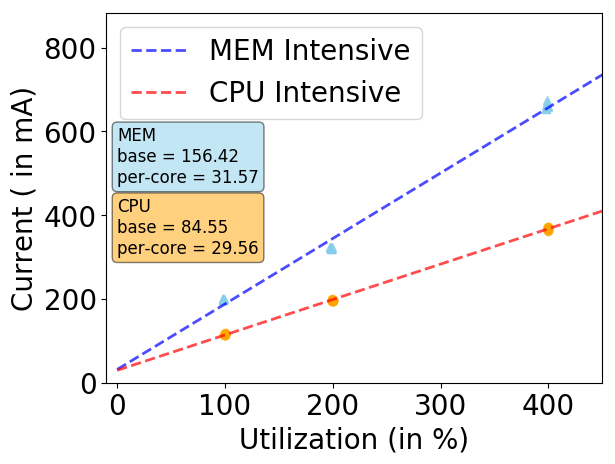
\includegraphics[width=\textwidth]{figures/1728000.png}
         \caption{1.728 GHz}
         \label{fig:cpu_1728000}
    \end{subfigure}
    \caption{The CPU derivation for two frequencies, 576 MHz and 1.728 GHz.}
    \label{fig:cpu_model_derivation}
    \vspace{-0.1in}
\end{figure}
\fi


\if 0
Figure~\ref{fig:cpu_model_derivation} shows 
the power consumed as a function of the CPU utilization for 576 MHz and 1.728 GHz,
for the two CPU benchmarks.
% While the blue line represents memory-intensive microbenchmark, red represents arithmetic-intensive microbenchmark .
% Figure~\ref{fig:cpu_576000} and~\ref{fig:cpu_1728000} corresponds to  576 MHz and 1.728 GHz
% Figure~\ref{fig:cpu_model_derivation} shows the power (averaged over 10 runs) linearly correlates with the utilization.
%% 3b. How model is derived
% We thus apply a regression-based solver to derive the best fit the following CPU power model:
% For each of the 31 frequencies, we derived a base and a per-core component with the following CPU power model.
% \begin{equation}
%     Power_{CPU}(f) = p_{base} + p_{f}*Utilization
% \end{equation}
% Where $p_{base}$ denotes the base power, and $p_{f}$ is the non-base per-core power running at frequency $f$.
%% 3c. Explain Base Current and Non-Base Current
For each of the 31 frequencies, we derived both base power and per-core component power.
We also observe that a reliable model can not be generated for the higher range of frequencies, like for frequencies higher than 2.035 GHz on MotoZ3 observations become unstable for CPU benchmarks.
The valid sets of base and per-core power were used for CPU modeling.
We observed that the base power is independent of frequency and per-core power is dependant on frequency.
Base power is 27.85 mA with a standard deviation of 1.22 mA.
% 
% We know the cores those are running at the 100\% utilization and remaining cores are offline.
% So, we can equate the number of running cores with utilization.
% We also observe that a reliable model can not be generated for the higher range of frequencies, like for frequencies higher than 2.035 GHz on MotoZ3 observations become unstable for CPU benchmarks.
% Fortunately, the apps rarely require these higher CPU frequency states and for our investigation we don't require those coefficients.
% \comment{stdev of what? fitting error on whole equation?}
% \comment{what is the following trying to say?}
During a  real run various cores may run on various frequencies.
\fi

\begin{figure}[tp]
    \centering
    \vspace{-0.1in}
         \begin{subfigure}[b]{0.49\columnwidth}
         \centering
    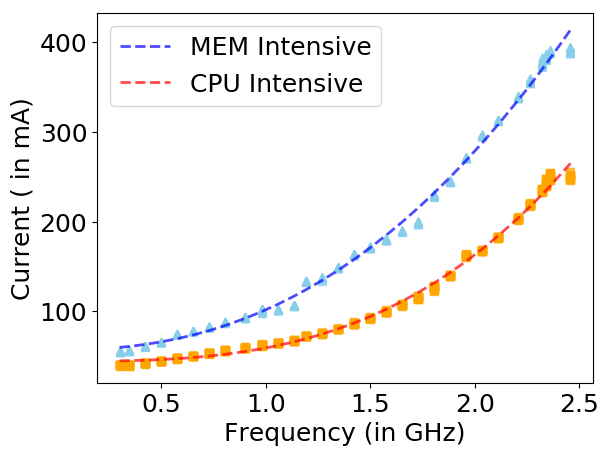
\includegraphics[width=\columnwidth]{figures/cpu_mem_characteristics.png}
    \caption{CPU power for compute-intensive vs. memory-intensive operations.}
    \label{fig:cpu_vs_mem}
\end{subfigure}
    \hfill
    \begin{subfigure}[b]{0.49\columnwidth}
         \centering
%    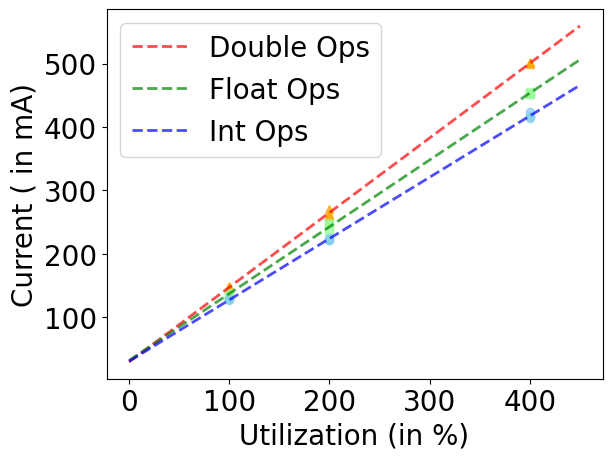
\includegraphics[width=\columnwidth]{figures/int_float_double.png}
    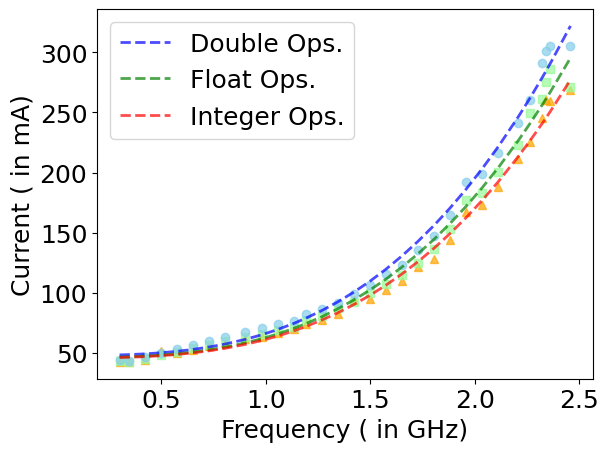
\includegraphics[width=\columnwidth]{figures/int_float_double_characteristics.png}
    \caption{CPU power for double, float and integer arithmetic operations.} % (for 1.8 GHz)}
    \label{fig:int_vs_float_vs_double}
    \end{subfigure}
    \caption{CPU power varies with app workload.}
    \label{fig:cpu_model_derivation}
    \vspace{-0.1in}
\end{figure}

\paragraph{Derived model}
Figure~\ref{fig:cpu_vs_mem} shows the derived CPU power model parameters
by plotting the total CPU power
as a function of the frequency.
% using the arithmetic-intensive and memory-intensive microbenchmarks. 
We observe that the CPU power draw for the two arithmetic-memory operation mix differ significantly,
by 38.7\% at the 300 MHz and 56.8\% at 2.45 GHz.
This suggests that the arithmetic-memory operation mix can send the CPU cores
to different power state variations draining different power.
In principle, this variation can be captured in the TPMD process by  
explicitly modeling memory as a separate phone component,
as in~\cite{carroll:2010,sesame:2011}, 
% gernot:2010 <- Koala: a platform for OS-level power management
using cache performance counter and free memory as the power triggers for memory draw. 
{
However, since the memory operation mix such as hardware counters is not collected by the mobile hardware 
or not reported by the Android OS on Android phones, it is much easier to lump memory power draw with CPU power draw as is commonly done in many recent work, including Android Battery Stats and Historian~\cite{androidbatterystats}. \comment{more example???}
}

Figure~\ref{fig:int_vs_float_vs_double} shows the derived CPU power model parameters for the integer only, 
float only, and double only arithmetic-intensive phases of the microbenchmark. 
We observe that the {CPU power} also differ, 
by 2.9\% at the 300 MHz and 13.5\% at 2.45 GHz.
This suggests that even the data type of arithmetic operations
can send the CPU cores into different power state variations.

\if 0
In summary, the above exercise of TPMD of CPU power shows the CPU power 
draw is very much app usage dependent and any fixed CPU model derived from
running a fixed microbenchmark is likely to have high estimation error when 
used in a particular app run. 
\fi


\if 0
\questionaj{This is not a very convincing argument. 1. For memory benchmark, is "CPU
power" = "CPU + memory" power? Or is the CPU power referenced in figure is true CPU 
power? If it is first, seeing higher "CPU power" is expected and not surprising.
2. Someone can argue that you could log memory triggers by instrumenting
compiler/libc/kernel,
why not just log?  Another paper didn't do it is not a strong reason. I think the 
argument we are trying to make is broader. That there are too many triggers that can 
affect a component power model. Because of which (a) micro-benchmark author may not 
know about all of them (b) building an exhaustive model could be expensive and not useful
as some model combinations may not even appear in real apps and (c) logging all 
triggers can be prohibitively expensive or not allowed. Because of this 
micro-benchmarks are hopelessly doomed.
If you agree,
we should also throw int-ops vs float-ops arithmetic, CPU temperature into the mix and use them to make the above three arguments.}
\fi
%\subsection{GPU Power Model is App Dependent}
\label{subsec:gpu}

Next, we show the GPU power model can also be highly dependent on app usage. 
The GPU gives an example of a component that cannot be exercised alone and we show
how TPMD models the GPU power incrementally over the CPU model.

%%% Things discussed in this section
%% 1. Explain GPU is complex in modern smartphones
%% 2. Explain the GPU frequencies and power states in modern smartphones
%% 3. Explain complete GPU model
%% 4. What did we do
%% 5. Explain results and observation
%%   5a. Explain per scenario dependent modeling
%%   5b. Explain the reasons for the observation

%The GPU of modern phones can run at various frequencies and transition among various power states.
\paragraph{Parameters of the GPU power model}
In Moto Z3, the GPU can run at 7 different frequencies and has three power states,
Active, Slumber (offline), and Aware.
When the GPU is woken out of the Slumber state, it enters the Aware state for a brief duration.
% \comment{Similarly, Nexus 6 can run at 5 different frequencies and three power states; Active, Init and Nap. Init corresponds to Aware and Nap corresponds to Slumber of Moto Z3}
%{
% How does does it stay in Aware?
%This the initialization phase of the GPU.
% for a fixed duration? 535 uS on average ( with a 250 uS difference between 435 uS (min) and 635 us (max))
% }
The Active state has two sub states, Active-busy when the GPU is computing and Active-idle
when the GPU is idle. After staying in Active-idle for a threshold interval, the GPU enters the Slumber state.
Since the GPU never enters the Slumber or Aware state when an app is running, 
the parameters of the GPU model include only the GPU power draw in Active-busy and Active-idle in each frequency, $p^g_{busy}(g_k), p^g_{idle}(g_k)$, as listed in Table~\ref{tab:parameters}.
We abbreviate Active-busy and Active-idle states simply
as GPU Busy and Idle states in the rest of the paper.

\if 0
Accordingly, we model the GPU power draw as follows:
\begin{equation}
    Power_{GPU} = \sum_{j}\sum_{i} u_{ij}*p_{ij}
    \end{equation}
where $p_{ij}$ is the power parameter for the $i^{th}$ GPU frequency for the $j^{th}$ power state (Active-busy, Active-idle, Slumber, Aware) and $u_{ij}$ is the corresponding utilization in that frequency and power state.
\fi

\paragraph{TPMD methodology}
% Similar to CPU, the GPU of modern smartphones have also vastly developed.
Initially, we tried to use a GPU benchmark, 3DMark~\cite{3DMark}, to drive the GPU usage into Busy and Idle states under each frequency.
However, we found that the GPU benchmark renders very different consecutive frames which
result in rapidly fluctuating GPU utilizations and power monitor readings.
This makes aligning the power monitor readings with the GPU Busy periods difficult
which is needed to extract the GPU Busy state power at each frequency.
%
% In power trace it was difficult to identify busy and idle traces for GPU benchmarks.This is because utilization is not constant as it continually generates new frames and can’t be paused.
% In apps the GPU utilization is constant because when no input is given to  the game app it generates the same frame again and again.
%
% we can only generate average GPU power coefficients for GPU busy and idle states.
% Average GPU coefficient depends on GPU utilization i.e  the time GPU is busy to total GPU running time.
%Average GPU power coefficients so derived is fixed and can not cater to two apps which may have different GPU utilization.
In contrast, we observe that real apps tend to render very similar consecutive frames in a short period of time which result relatively stable GPU utilization and stable GPU power draw, 
making it much easier to extract the power monitor reading corresponding to a given GPU utilization
(see Figure~\ref{fig:power_trace_candycrushturorial} later). 
%  the rendering task often finishes in less than the 16.7ms per-frame interval and hence the GPU will go through busy and idle states in every 16.7ms interval, making it much easier to manually identity both states. 
% \questionaj{Why do we have to identify manually? Triggers are not available in atrace?
% Due to both drift and scaling their is vast alignment problem in aligning each 16.7 ms interval.
% Alignment problem prevent us from directly using triggers from the event trace.}
Based on this observation, we directly used selected apps that use 
only the CPU and GPU to derive the GPU power models. 
In particular, we derive the CPU model first using the integer-arithmetic microbenchmark\footnote{We found using the CPU model derived using memory-intensive microbenchmark
resulted in negative GPU coefficients.}
and then use the difference 
between the measured phone power and model-estimated CPU power as the ground-truth for the GPU power draw
in GPU power model derivation.


% 5. Explain results and observation

\begin{table*}[tp]
{\footnotesize
    \centering
    \caption{Moto Z3 GPU power model (Busy and Idle power per frequency) with the CPU fixed at 1.056 GHz.}
    \vspace{-0.1in}
    \begin{tabular}{|p{11.5mm}|p{22mm}|c|c|c|c|c|c|c|c|c|c|c|c|c|c|}
    \hline
    App & Scenario & \multicolumn{14}{c|}{GPU Frequency} \\
    \cline{3-16}
     &  & \multicolumn{2}{c|}{257 MHz} & \multicolumn{2}{c|}{342 MHz} & \multicolumn{2}{c|}{414 MHz} & \multicolumn{2}{c|}{515 MHz} & \multicolumn{2}{c|}{596 MHz} & \multicolumn{2}{c|}{670 MHz} & \multicolumn{2}{c|}{710 MHz} \\
     \cline{3-16}
     & & Busy & Idle & Busy & Idle & Busy & Idle & Busy & Idle & Busy & Idle & Busy & Idle & Busy & Idle \\
    \hline
       \multirow{3}{11mm}{Boat Racing}  & Intro & 208.5 & 134.7 & 253.7 & 67.25 & 283.2 & 149.9 & 423.6 & 124.5 & 581.6 & 79.85 & 633.2 & 162.2 & 703.2 & 184.2 \\
       \cline{2-16}
        & Still & 232.3 & 145.5 & 358.0 & 57.00 & 402.8 & 153.0 & 573.9 & 92.17 & 576.3 & 150.0 & 813.9 & 145.0 & 866.3 & 205.9 \\
         
         & GPU engy. error (\%) & 232.3 & 145.5 & 358.0 & 57.00 & 402.8 & 153.0 & 573.9 & 92.17 & 576.3 & 150.0 & 813.9 & 145.0 & 866.3 & 205.9 \\
         
         \hline
        \multirow{2}{11mm}{Bricks Breaker}  & Intro & 140.7 & 70.33 & 158.3 & 69.32 & 204.3 & 109.9 & 166.8 & 134.4 & 130.0 & 141.3 & 115.5 & 172.9 & 133.2 & 191.4 \\
       \cline{2-16}
         & Still & 180.8 & 72.69 & 185.5 & 72.63 & 177.7 & 113.0 & 243.6 & 112.8 & 271.3 & 115.6 & 375.7 & 138.1 & 441.2 & 154.7 \\
         \hline
        \multirow{2}{13mm}{Candy Crush Saga}  & Into & 228.0 & 83.88 & 262.5 & 83.97 & 344.4 & 112.7 & 523.1 & 123.3 & 620.7 & 120.0 & 792.6 & 146.2 & 900.4 & 167.2 \\
        \cline{2-16}
         & Tutorial & 226.3 & 92.85 & 228.4 & 89.50 & 330.6 & 117.7 & 445.2 & 134.5 & 519.6 & 137.5 & 660.2 & 160.7 & 855.3 & 171.6 \\
         \hline
    \end{tabular}
    \label{tab:gpumodel_motoz3}
    \vspace{-0.1in}
    }
\end{table*}

% Comparison Table for GPU model with other scenarios Here

We repeated the GPU model derivation for three
popular games apps, Boat Racing, Candy Crush Saga and Bricks breaker.
each running two scenarios, as listed in Table~\ref{tab:app_scenario_description}.
To minimize the variance of CPU power draw, we fixed the CPU frequency at 1.056 GHz,
and ran each app scenario under each GPU frequency for a duration of 60 seconds.

\paragraph{Derived model}
Table~\ref{tab:gpumodel_motoz3} shows the derived GPU power models for varying GPU frequencies for Moto Z3 and Table~\ref{tab:gpumodel_nexus6} for Nexus 6.
%% 5a. Explain per scenario dependent modeling
We make two observations.
(1) The GPU power parameters for the same frequency differ with {\it different apps}; at 710 MHz, the GPU Busy power draw for Boat Racing is 10.6\% lower than for Candy Crush Saga on Moto Z3.
(2) The GPU parameters for the same frequency even differ for {\it different scenarios} 
of the same app; for Boat Racing, the GPU Busy power draw
for the Intro scenario is 10.2\% and 29.7\% lower than for the Still scenario
at 257 MHz and 414 MHz, respectively.

To show the importance of app-specific power modeling, we calculated the error
in estimating the total GPU energy drain in the second scenario of each app 
if using the GPU model derived using the first scenario of each app.
Table~\ref{tab:gpumodel_motoz3} shows that the error ranges between 
??\%--??\%, ??\%--??\%, and ??\%--??\% for the second scenarios of the three apps.


%% 5b. Explain the reasons for the observation
The above dependence of the GPU power draw on app usage can be attributed  to two main reasons.
First, the GPU has a large number of mini-cores, but the utilization metric available to the OS only captures the temporal utilization but not the spatial utilization, \ie the percentage of mini-cores that were active.
Different spatial utilization may drive the GPU into different power state variations that have the same temporal utilization but different power draw.

Second, rendering different frames in different scenarios of the same app or different apps may result in different memory operation mix, and hence using a single CPU model in estimating the CPU power draw portion to be subtracted from the total phone power 
may result in errors in the GPU power draw  estimation, as we see in \S\ref{sec:primer_cpu}. 
Such error propagation happens in TPMD which models one component at a time
and often relies on the models for prior components to estimate the "ground truth" in modeling  the next component. 

\subsection{TPMD is labour intensive}

\paragraph{Designing microbenchmarks} 
We start the process of TPMD by first identifying the list of {\it power model parameters}
for CPU and GPU, as listed in Table~\ref{tab:parameters}.
% \paragraph{Parameters of the CPU and GPU power models.}
% Pixel2, Moto Z3~\cite{motoz3} and Pixel 4 are representative of modern smartphones
% that uses the big.LITTLE CPU architecture~\cite{biglittlearch} to
% provide energy efficiency in supporting diverse workloads.
% Particularly, in Pixel 2 and Moto Z3, the LITTLE cores can operate in 22 different frequencies 
% and big cores can operate in 31 different frequencies.
% Whereas, for Pixel 4, the LITTLE cores can operate in 18 different frequencies 
% and big cores can operate in 20 different frequencies.
%  The cores are switched to higher frequencies when higher performance is required.
% At runtime, the OS scheduler along with the CPU governor performs power state transition and core frequency scaling to optimize the CPU energy draw as the workload varies.
From~\cite{multicoremodel:2015}, the parameters of the CPU power model include
the base power consumed $p_{\text{base}}$ when the cores are idle and
the non-base core $i$ power running at frequency $f_k$, $p^c_i(f_k)$.
%, as listed in Table~\ref{tab:parameters}.
% The total CPU power can be modeled as:
% {
% \begin{equation}
%     P_{\text{CPU}} = p^c_{\text{base}} + \sum_{i} p^c_i(f_k)
% \end{equation}
% 
% }
% In Moto Z3, 
% GPU can run at different frequencies and can either be busy or idle.
% has three power states, Active, Slumber, and Aware.
% Since the GPU never enters the Slumber or Aware state when an app is running, 
The parameters of the GPU model include the GPU power draw in 
% Active-busy and Active-idle 
busy and idle states in each frequency, $p^g_{\text{busy}}(g_k)$ and 
$p^g_{\text{idle}}(g_k)$.
% We abbreviate Active-busy and Active-idle states simply
% as GPU Busy and Idle states in the rest of the paper.

% \if 0
% Accordingly, we model the GPU power draw as follows:
% \begin{equation}
%     Power_{GPU} = \sum_{j}\sum_{i} u_{ij}*p_{ij}
%     \end{equation}
% where $p_{ij}$ is the power parameter for the $i^{th}$ GPU frequency for the $j^{th}$ power state (Active-busy, Active-idle, Slumber, Aware) and $u_{ij}$ is the corresponding utilization in that frequency and power state.
% \fi

%\paragraph{TPMD methodology.}
We design CPU microbenchmarks that perform 
arithmetic and memory operations for 7 seconds each 
with 100\% utilization.

\begin{sloppy}
For the GPU, we first used a third-party rendering benchmark 3DMark~\cite{3DMark}. 
	But on running the benchmark, we found that 3DMark renders quite different
	consecutive frames which result in rapidly fluctuating GPU utilizations and
	power monitor readings, making the alignment \comment{of what?? of
	the 16.7 ms GPU rendering intervals wrt the power monitor as each rame has a different GPU utilization} difficult. 
\end{sloppy}
In contrast, we observed that real apps tend to render very similar consecutive
frames in a short period of time which result in relatively stable GPU
utilization and stable total power draw, making it easier to extract the power
monitor reading corresponding to a given GPU utilization (see
Figure~\ref{fig:power_trace_candycrush_menu} later).  Thus, we directly used
selected apps that use only the CPU and GPU to derive the GPU power models.  In
particular, we derive the CPU model by first using the 
% integer-arithmetic 
CPU arithmetic microbenchmark\footnote{We found using the CPU model derived
using memory-intensive microbenchmark resulted in negative GPU coefficients.}
and then using the difference between the measured phone power and
model-estimated CPU power when running an app as the ground-truth for the GPU
power draw and GPU power model derivation.


\paragraph{Running microbenchmarks}
\aj{We first prepared the three phones by connecting power monitor and bypassing 
the battery interface.} \comment{Were there some challenges here for separate 
device models?}
\dcomment {
We faced different challenges while attaching each device to the power monitor
\eg attaching the power monitor leads to power management circuit .
}

We ran the CPU microbenchmark while fixing the big core cluster at each 
of the 31 frequencies
for both Pixel 2 and Moto Z3 and at each of the 20 frequencies for Pixel 4, 
on 1 core and 2 cores.
% When using 1 core, 2 cores and 4 cores, the remaining cores are offline.
We measure the base CPU power as the phone power draw when all cores are idle.
We manually align the power monitor readings for each of the 7-second interval 
and derive the non-base per-core power for each frequency by 
subtracting the base power from the measured total phone power.
\comment{This is not bad? Only (7+7)*31 = ~7 minutes of run. Do we have to repeat
it multiple times or something else that makes it LABORIOUS?
}
\dcomment{
For the purpose for this paper we considered only 2 big cores for the ease of our experiments.
While in the real world scenario the device has to profiled on all states \ie
taking into account the interaction between the LITTLE core and big cores.
There are in total 24 configuration of cores for Pixel 2 in which they can be
online ( for a 4 LITTLE cores 0 to 4 cores could be active, same for big cores,
remove the case where both cores are offline).
As there are 22 LITTLE core and 31 big core frequencies we further have $22x31=682$
combination. Using our methodology it could take up to $24x682x7$ seconds = 1.33 days for
just to gather the required measurements.
}
% After running
% the benchmarks, we found that for all the
% phones, 
% %we found that 
% the per-core power $p_i(f_k)$ remains the same for different cores.

% Similar to CPU, the GPU of modern smartphones have also vastly developed.
% Initially, we tried to use a GPU benchmark, 3DMark~\cite{3DMark}, to drive the GPU usage into Busy and Idle states under each frequency.
%
% This makes aligning the power monitor readings with the GPU Busy periods difficult
% which is needed to extract the GPU Busy state power at each frequency.
%
%  the rendering task often finishes in less than the 16.7ms per-frame interval and hence the GPU will go through busy and idle states in every 16.7ms interval, making it much easier to manually identity both states. 
% \questionaj{Why do we have to identify manually? Triggers are not available in atrace?
% Due to both drift and scaling their is vast alignment problem in aligning each 16.7 ms interval.
% Alignment problem prevent us from directly using triggers from the event trace.}

% 5. Explain results and observation

\begin{figure*}[tp]
    \centering
     \begin{subfigure}[b]{0.32\textwidth}
         \centering
         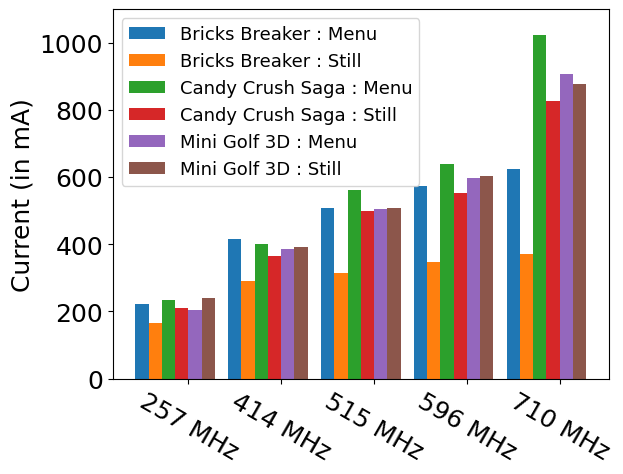
\includegraphics[width=\textwidth]{figures/002_Pixel2_gpu_model.png}
         \caption{Pixel 2}
         \label{fig:gpu_model_p2}
     \end{subfigure}
    \begin{subfigure}[b]{0.32\textwidth}
         \centering
         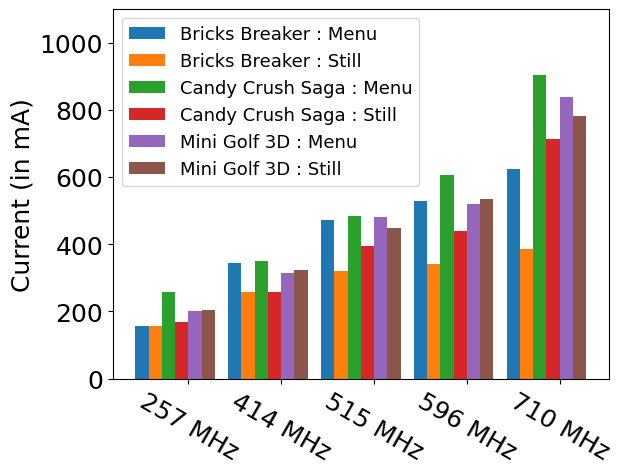
\includegraphics[width=\textwidth]{figures/003_MotoZ3_gpu_model.png}
         \caption{Moto Z3}
         \label{fig:gpu_model_z3}
     \end{subfigure}
    \begin{subfigure}[b]{0.32\textwidth}
         \centering
         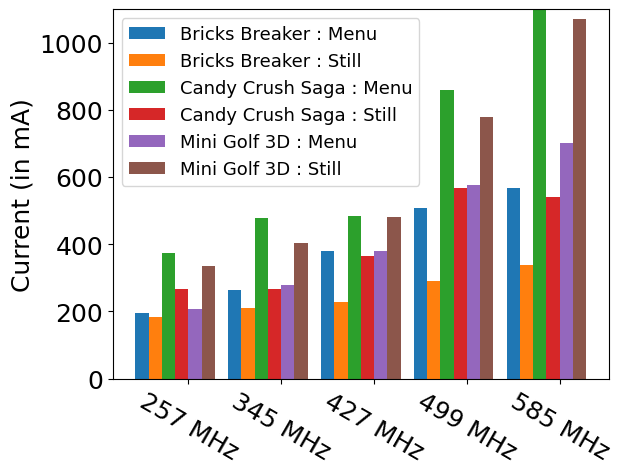
\includegraphics[width=\textwidth]{figures/004_Pixel4_gpu_model.png}
         \caption{Pixel 4}
         \label{fig:gpu_model_p4}
     \end{subfigure}
     \hfill
    \caption{TPMD-derived GPU power model (only Busy power is shown) with
        the CPU frequency fixed at 1.42 GHz for both Pixel 2 and Moto Z3,
        and 1.61 GHz for Pixel 4. ??? FIXED}
    \label{fig:gpu_model}
    \vspace{-0.1in}
\end{figure*}

\begin{table*}[tb]
    \caption{Energy estimation error (\%) for app scenarios 
    using the GPU model derived for each scenario with CPU and GPU frequencies fixed for the 3 phones. (B: Bricks Breaker, C: Candy Crush Saga and M: Mini Golf 3D)}
    \vspace{-0.1in}
    \centering
    \begin{subfigure}[b]{0.31\textwidth}
        \caption{Pixel 2}
        \vspace{-0.05in}
        \centering
    	{ \scriptsize
    	\begin{tabular}{ | p{10.8mm} | c | c | c | c | c | c | }
    		\hline
    		     & \multicolumn{6}{ c|}{Error for each App Sc. (\%)}\\ % \multicolumn{6}{ c|}{Error for each App Scenarios (\%)}\\
    		\cline{2-7}
                    Model & \rot{B. Menu} & \rot{B. Still} & \rot{C. Menu} & \rot{C. Still} & \rot{M. Menu} & \rot{M. Still}  \\
    		\hline
                B. Menu              & 8.9 & 13 & 20 & 16 & 11 & 14 \\
                B. Still             & 15 & 11 & 31 & 25 & 17 & 26 \\
                C. Menu              & 16 & 24 & 11 & 11 & 13 & 11 \\
                C. Still             & 16 & 19 & 14 & 12 & 12 & 14 \\
                M. Menu              & 9.9 & 14 & 14 & 11 & 8.1 & 11 \\
                M. Still             & 12 & 21 & 9.7 & 10 & 11 & 8.6 \\
    		\hline
    	\end{tabular}
    	}
    \end{subfigure}
    \hfill
    \begin{subfigure}[b]{0.31\textwidth}
        \caption{Moto Z3}
        \vspace{-0.05in}
        \centering
    	{ \scriptsize
    	\begin{tabular}{ | p{10.8mm} | c | c | c | c | c | c | }
    		\hline
    		     & \multicolumn{6}{ c|}{Error for each App Sc. (\%)}\\ % \multicolumn{6}{ c|}{Error for each App Scenarios (\%)}\\
    		\cline{2-7}
                    Model & \rot{B. Menu} & \rot{B. Still} & \rot{C. Menu} & \rot{C. Still} & \rot{M. Menu} & \rot{M. Still}  \\
    		\hline
                B. Menu              & 16 & 18 & 44 & 18 & 22 & 25 \\
                B. Still             & 18 & 15 & 36 & 15 & 17 & 17 \\
                C. Menu              & 30 & 24 & 16 & 23 & 18 & 16 \\
                C. Still             & 12 & 12 & 31 & 11 & 15 & 17 \\
                M. Menu              & 18 & 16 & 23 & 15 & 14 & 15 \\
                M. Still             & 20 & 15 & 20 & 14 & 12 & 13 \\
    		\hline
    	\end{tabular}
    	}
    \end{subfigure}
    \hfill
    \begin{subfigure}[b]{0.31\textwidth}
        \caption{Pixel 4}
        \vspace{-0.05in}
        \centering
    	{ \scriptsize
    	\begin{tabular}{ | p{10.8mm} | c | c | c | c | c | c | }
    		\hline
    		     & \multicolumn{6}{ c|}{Error for each App Sc. (\%)}\\ % \multicolumn{6}{ c|}{Error for each App Scenarios (\%)}\\
    		\cline{2-7}
                    Model & \rot{B. Menu} & \rot{B. Still} & \rot{C. Menu} & \rot{C. Still} & \rot{M. Menu} & \rot{M. Still}  \\
    		\hline
                B. Menu              & 15 & 15 & 44 & 19 & 15 & 34 \\
                B. Still             & 15 & 15 & 50 & 23 & 17 & 40 \\
                C. Menu              & 30 & 33 & 12 & 20 & 25 & 13 \\
                C. Still             & 18 & 20 & 25 & 15 & 16 & 19 \\
                M. Menu              & 15 & 16 & 34 & 17 & 14 & 26 \\
                M. Still             & 25 & 28 & 13 & 15 & 21 & 12 \\
    		\hline
    	\end{tabular}
    	}
    \end{subfigure}
    \label{tab:gpu_model_error}
    \vspace{-0.1in}
\end{table*}
% Comparison Table for GPU model with other scenarios Here

For GPU model derivation, we repeated runs for three popular games apps,
Bricks Breaker, Candy Crush Saga and Mini Golf 3D, each running two
scenarios, as listed in Table~\ref{tab:app_scenario_description}.  To
minimize the variance of CPU power draw, we fixed the CPU frequency at
1.42 GHz for both Pixel 2 and Moto Z3, and 1.61 GHz for Pixel 4, and ran
each of the app scenario under each GPU frequency for a duration of 30
seconds.
\comment{Again, not not bad. What makes this process LABORIOUS?}
\dcomment {
The GPU model derivation has to be derived for each app the user requires.
Making this impossible to device manufactures to model GPU in it entirely
as there are billions of apps presents currently.
}

\subsection{TPMD is not comprehensive}

Our CPU modeling results (details omitted) show that
the CPU power draw for the arithmetic-intensive and memory-intensive
operations of the microbenchmark differ significantly,
by 38.7\% at 300 MHz and 56.8\% at 2.45 GHz for Moto Z3.
This suggests that the arithmetic-memory operation mix can send the CPU cores
to different power state variations, draining different amount of power.

Figure~\ref{fig:gpu_model}(a)-(c) shows the derived power models 
for varying GPU frequencies for the 3 phones. 
Only GPU Busy power are shown due to page limit.
% The full bars represent the busy current whereas the solid bars are the idle current.
% and Table~\ref{tab:gpumodel_nexus6} for Nexus 6.
%% 5a. Explain per scenario dependent modeling
We make two observations.
%
(1) The GPU power parameters for the same frequency differ with {\it
different apps}. For example, on Moto Z3 at 710 MHz, the GPU Busy power draw for
Bricks Breaker Still is 57.2\% lower than for Candy Crush Saga Menu.
%
(2) The GPU power parameters for the same frequency even differ for
{\it different scenarios} of the same app. For example, for Bricks Breaker, the GPU
Busy power draw for the Still scenario is 32.3\% and 35.5\% lower than
for the Menu scenario at 515 MHz and 596 MHz, respectively, on Moto Z3.
Similar observations can be made about the other two phones.

%% 5b. Explain the reasons for the observation
The above dependence of the GPU power draw on app usage can be
attributed to two main reasons.  (1) The GPU has a large number of
mini-cores, but the utilization metric available to the OS only
captures the temporal utilization and not the spatial utilization, \ie
the percentage of mini-cores those were active.  Different spatial
utilization may drive the GPU into different power state variations
that have the same temporal utilization but different power draw.
% 
(2) Using a single CPU model in estimating the CPU power draw which is
 to be subtracted from the total phone power may result in errors in
 the GPU power draw estimation, as rendering different frames for
 different app scenarios (of the same or different apps) may result in
 different CPU usage, \eg due to different mix of arithmetic and
 memory operations and hence CPU power draw.  Such error propagation
 happens in TPMD which models one component at a time and often relies
 on the models of a prior component to estimate the "ground truth" in
 modeling the next component.

% \paragraph{Cross validation.}
To further demonstrate that the GPU models derived per app scenario captures
the model dependence on the app usage also, we perform a cross validation
by applying the GPU model derived from each of the six app scenarios
shown in Figure~\ref{fig:gpu_model}(a)-(c) to estimate the total
energy of all app scenarios (including self).
Tables~\ref{tab:gpu_model_error}(a)-(c) shows the results for 
the case where the CPU frequency is fixed at 1.42 GHz for Pixel 2 and Moto Z3 and 1.61 GHz for Pixel 4, and the GPU frequency is fixed at 257 MHz for all three phones.
We observe that the energy estimation error
is much lower when the GPU model derived for an app scenario is
applied to itself (diagonal values), ranging between 
8.09\%-11.56\% for Pixel 2,
11.47\%-16.25\% for Moto Z3, and
11.90\%-15.21\% for Pixel 4,
than when a model derived for one scenario is applied
to other scenarios (off-diagonal values), which
range between 
9.73\%-31.26\%,
11.57\%-44.25\%, and
13.07\%-50.43\%.


% \comment{
% We observe that the lowest error for a scenario is
% due to GPU model derived from same scenario (fitting error), whereas for
% all other scenario GPU models the error can be as much as 2$times$ higher.
% For the higher GPU frequencies, like 710 MHz the difference in the can increase up to about 10 times.
% }


\if 0
we calculated the error
in estimating the total GPU energy drain in the second scenario of each app 
if using the GPU model derived using the first scenario of each app.
The rows labelled "GPU energy error" in Table~\ref{tab:gpumodel_motoz3} shows that the error ranges between ??\%--??\%, ??\%--??\%, and ??\%--??\% for the second scenarios of the three apps.
\fi







\paragraph{Summary.}
The above exercise of applying TPMD to derive the CPU and GPU models for 3 phones
have two important implications.
%
(1) TPMD is a laborious time-consuming process. In-situ power modeling
such as done by SPMD will enable rapid portability of energy related software.
(2) The GPU power draw is very much dependent on app usage; different
app usage can lead to variations of the same power state that draw
different amount of power. Hence {\it any fixed GPU model derived from
running a particular microbenchmark or app is likely to have high
estimation error when it is applied for a different app run.} This
motivates the need for SPMD which is inherently app usage specific.
%
\comment{(3) Don't think this should be here. This section is about TPMD. Find where to
move it.
Since different scenarios of the same app can drive components
into different power state variations, {\it the equations from
different scenarios of the same app run should not be grouped into the
same system of equations to be fed into the solver in SPMD,} as this
defeats the app usage specificity nature of SPMD.}

